\documentclass[10pt,twocolumn]{article}
\usepackage{graphicx}
\usepackage{times}
\usepackage{url}
\usepackage{fancyhdr}
\usepackage{tabularx}
\usepackage{hhline}
\usepackage{color}
\usepackage{alltt}
%\usepackage{draftcopy}
\usepackage{xspace}
\usepackage{cite}
%\usepackage{parskip}

\setlength{\voffset}{0in}
\setlength{\hoffset}{0in}
\setlength{\headheight}{0pt}
\setlength{\topmargin}{-.25in}
\setlength{\oddsidemargin}{0in}
\setlength{\evensidemargin}{0in}
\setlength{\textheight}{9in}
\setlength{\textwidth}{6.5in}
\setlength{\headsep}{.25in}
% \setlength{\columnsep}{0.11in}
\newlength{\figurewidth}
\setlength{\figurewidth}{\columnwidth}
\def\graphscale{.88}
\linespread{0.988}

\renewcommand{\subsection}[1]{\vspace{10pt}\noindent\textbf{#1:}\vspace{5pt}}
%\markboth{Draft}{Preprint--Please do not redistribute}
\pagestyle{myheadings}

%% The name of the system is....?
\def\Sys{P2\xspace}
\def\Lang{OverLog\xspace}
\def\ELang{PEL\xspace}
\def\Elang{\ELang}
\def\PChordLines{33\xspace}
\def\MacChordLines{320\xspace}
\def\PNaradaLines{12\xspace}

\renewcommand{\ttdefault}{cmtt}
\newenvironment{overlog}{\begin{alltt}\small}{\end{alltt}}

%\newcommand{\note}[1]{[{\textit{#1}}]}
%\newcommand{\note}[1]{[\textcolor{red}{\textit{#1}}]}
\newcommand{\note}[1]{}

\bibliographystyle{abbrv}
\let\oldthebibliography=\thebibliography
\let\endoldthebibliography=\endthebibliography
\renewenvironment{thebibliography}[1]{%
    \begin{oldthebibliography}{#1}%
    \setlength{\parskip}{0ex}%
    \setlength{\itemsep}{0ex}%
}%
{%
    \end{oldthebibliography}%
}

\begin{document}

\title{Finally, a Use for Componentized Transport Protocols}
\author{Tyson Condie, Joseph M. Hellerstein, Petros Maniatis, Sean
  Rhea, Timothy Roscoe \\
U.C. Berkeley and Intel Research Berkeley}
\date{}
\maketitle
\thispagestyle{plain}

%{\footnotesize
%\begin{verbatim}
%$Id: paper.tex,v 1.87 2005/10/27 08:43:53 troscoe Exp $
%\end{verbatim}
%}
\begin{abstract}
This paper argues a new relevance for an old idea: decomposing
transport protocols into a set of resuable building blocks that can be
recomposed in different ways depending on application requirements.
We conjecture that point-to-point applications may well be adequately
served by the existing suite of monolithic protocol implementations,
but widely-distributed peer-to-peer systems such as overlays are not:
the design space of transport protocols between nodes in a
large, highly coordinated system is much larger.  We provide several
examples of existing systems that have implemented a diverse range of
transport protocols, and show how a building-block approach covers
these systems well, enabling simple specification of hybrids and
variants of the protocols.  In particular, we show how all of our examples 
can be implemented in the networking stack of P2, a multipurpose system for
building overlay networks from declarative specifications. 

%% Academics have long argued for the need of a flexible transport layer
%% that can be tailored to the application needs and the network
%% technology underneath. A vast amount of research has gone into the
%% design of flexible, easy to configure, network protocols. However,
%% much of this work did not make it into the mainstream since most
%% application needs, at the time, were satisfied by the monolithic
%% network services provided by the kernel. Many recent applications are
%% using Overlay networks as a communication medium. Overlay networks
%% have a number of unique properties including routing freedom,
%% unpredictable next hops and node session times, and message buffering
%% and transformation alternatives.

%% The "one size fits all" network protocols of the past are not well
%% suited to handle the rich set of options intrinsic to Overlay
%% networks. In this paper, we revisit the idea of componentized
%% protocols in light of the growing need for Overlay network
%% support. Our definition of a component is a small processing unit that
%% performs some action on the traffic that traverses it. We connect such
%% components (elements) together using a dataflow graph, which is an
%% abstraction that provides ample flexibility in creation of network
%% protocols, as demanded by Overlay network architectures.

\end{abstract}

% % % % % % % % % % % % % % % % % % % % % % % % % % % % % % % % % % 
\section{Introduction}
\label{sec:intro}

\note{Outline: This is a topic of long interest.}

There has been a steady stream of research over the years into
\emph{componentized protocols}: protocol 
implementations assembled from a variety of building blocks.  A 
promise of such frameworks has generally been
flexibility: a protocol stack tailored for a particular application
can be easily assembled, usually without writing any new code, by
binding protocol objects together. 

\note{Outline: But the interest has yet to translate to application.}

Despite its conceptual elegance, protocol
implementations based on this approach have never
caught on, particularly at the transport level.  Most
applications today use a
kernel-provided IP stack, and usually TCP for transport.  The consensus is that 
for both bulk-transfer of data and RPC-like call semantics, TCP appears to be
perfectly adequate, and it is not worth inventing something new.

\note{Outline: The few possible applications are niche.}

Of course, a few applications have been identified where a radically different
transport protocol is appropriate, and in these cases a
new, complete, and different protocol has been devised
(e.g. RTP~\cite{rfc:1889}  for multimedia, or SCTP~\cite{rfc:2960}
for PSTN-like signalling traffic) rather than composing a protocol
from building blocks.  The use of these standard protocols has further
diminished the motivation for  transport protocols whose functionality
can be composed at user level in an application-specific manner.  

\note{Outline: Summing up the lack of applicability.}

We suspect that this small set of transport protocols (along with
DCCP~\cite{dccp-problem}) covers the needs of almost all
point-to-point applications; that is, applications based on the
concept of two end-points communicating. 

\note{Outline NOW, the payoff for the promise of the title.}

However, in this paper we argue that widely-distributed systems,
including structured and unstructured overlays, change this situation
and introduce problems that componentized transport protocol
mechanisms are uniquely equipped to solve.  

\note{Paper outline Part 1: look at new apps with custom transport} 

In the last few years,
considerable research has been devoted to both structured and
unstructured \emph{overlay} and \emph{peer-to-peer} applications.  As
distributed systems, these applications generally include their own
techniques for routing messages on an overlay.   Many such deployed
systems, including Bamboo~\cite{rhea_usenix_2004}, MIT
Chord~\cite{chord}, and P2~\cite{p2:sosp}, use custom transport protocols which provide
 TCP-friendly congestion control behavior, but over UDP.

\note{Paper outline 2: What's different in the apps?  What's required
  of the transport?}  
In Section~\ref{sec:whatsdifferent}, we attempt to explain this design
shift by 
examining features of P2P applications and overlays that
motivate their designers to adopt custom transport protocols, and the
way in which these applications differ from traditional network-based
applications.  With examples from specific applications, we
highlight more generic requirements for transporting data in these
settings.

\note{Paper outline 3:  Flexible is required.}  In the
end, however, our message is not simply that the features of modern
distributed systems require a rethinking of transport protocols.  We
also argue that these features greatly widen the design space for such
protocols and require an ability to easily customize transport
protocols for various distributed applications.  

To support this argument, we describe the transport protocol portion
of P2, a declarative overlay processor we have built~\cite{p2:sosp}.
P2 allows custom transport protocols to be assembled
from reusable dataflow building blocks. We show how a
variety of diverse but important application behaviors can be 
achieved naturally within P2's framework, in ways that are hard
or impossible to achieve with monolithic kernel implementations of
transport protocols such as TCP, RTP, SCTP or DCCP. 

% % % % % % % % % % % % % % % % % % % % % % % % % % % % % % % % % % 
\section{What's different?}
\label{sec:whatsdifferent}

%What is different about the P2P applications observed to be using UDP
% to transfer significant amounts of data?   
We have asserted that new, distributed, UDP-based applications behave
in ways that are not well served by traditional transport protocols.
In this section we identify several
features of such applications that distinguish them from, say, typical
web services.   

First we note that at a node-to-node level, P2P
communication often requires different subsets of the TCP
functionality set---in-order delivery, reliability, congestion
control. 
DCCP~\cite{dccp-problem} explicitly addresses this design space,
defining an additional kernel datagram protocol providing
congestion control and flexible packet acknowledgement. 

However, in this paper we argue that a more general approach than DCCP
is required.  We present use-cases in P2P systems where
implementation is not possible using DCCP, and cases which
require substantial implementation in addition to DCCP.   While most
of our examples are from structured P2P overlays, we stress that the
principles here are by no means limited to the DHT space. 
We also note that DCCP is a protocol rather than an
implementation per se.  The question of whether DCCP itself is
naturally implementable within the framework of section~\ref{sec:p2}
is beyond the scope of this paper.

Some of our example distinctions below relate to desired protocol
\emph{behavior}, while others concern the design of a suitable protocol
\emph{API} for end-systems.  However, both affect how the protocol is implemented.

% % % 
\subsection{Application-level routing freedom}
\label{sec:routingFreedom}
% % % 

Widely-distributed applications have many choices about
where to forward a message.  Unlike traditional client-server
applications, there may be several equivalent end-points for a message 
(e.g., to retrieve a replica of some object).  
Moreover, P2P systems usually incorporate some kind of overlay
network, even if it is not explicit in the
design (e.g., the structured overlay of a DHT, or the
link-state overlay of an enterprise network of Microsoft
Exchange servers).  This provides options not only for the
destination of a message, but also the overlay path taken to get
there.

Designers exploit this new-found freedom to achieve high performance
(latency, throughput, reliability, etc.) by implementing
sophisticated adaptive policies for forwarding data in the system.  For
example, a node in the Bamboo DHT~\cite{rhea_usenix_2004} constantly
measures minimum round-trip times to nodes in its routing table, sets
aggressive timeouts, and rapidly resends messages to alternate
neighbors if these timeouts are exceeded.   This performs
dramatically better under churn, since Bamboo can rapidly route 
around failures and transient load spikes~\cite{rhea_usenix_2004}. 

In terms of the implementation, this inverts a
traditional ordering of functionality in a transport stack:
destination selection (e.g., the lookup in Bamboo's routing table)
now takes place downstream of retries, since successive
retries for a message can be sent to different destinations. 

\subsection{Congestion control aggregation}

\label{sec:unpredictableNextHop}
In addition to having flexibility in the choice of destination, some
P2P applications have the additional property of choosing among a very
large set of such destinations---a set whose size and contents are
typically not known in advance.  A good example
is the iterative routing employed by MIT
Chord~\cite{dabek_nsdi04} and the Kademlia~\cite{kademlia} variants used in
eDonkey~\cite{edonkey} and trackerless BitTorrent~\cite{bittorrent-dht}.  

A problem thus arises maintaining congestion windows for a
large and unpredictable number of destinations, many of which are only
needed for a single lookup RPC.  To address this problem,
DHash++ uses a custom transport protocol called
STP~\cite{dabek_nsdi04} that maintains aggregate congestion state for
all nodes, rather than the per-node state maintained by TCP, DCCP, etc. 
Consequently, all outgoing packets traverse a single
congestion-control instance before being sent to a variety of
destinations. 

This technique represents a different change in the
transport stack implementation from the Bamboo example above.  Here,
congestion control is performed independently of the destination of
messages.  Indeed, the decision of where to send the message may be
deferred until the congestion window allows it to be sent. 

% % %
\subsection{Application buffer management}
\label{sec:applicationBufferManagement}
% % %

The designers of DCCP point out the benefits to applications of
``\emph{late data choice}, where the application commits to sending a
particular piece of data very late in the sending
process''~\cite{dccp-api} and suggest using familiar ring-buffer
techniques for queueing packets rather than the traditional Unix API.
This change allows latency-sensitive applications to revise or replace
outgoing packets up until the time when the protocol
implementation can send them. 

A good motivating example is the use of in-network
aggregation techniques for disributed query processors such as
PIER~\cite{pier-cidr} and ~\cite{Yalagandula2004}.  Data is sent
up an aggregation tree to the
root, and aggregation computation is performed at any intermediate
node holding more than one datum at a time.  Ideally, each node
would send data up the tree eagerly (whenever congestion
control allowed it), but otherwise aggregate it with any new data
arriving from below. 

In practice, traditional protocol implementations
(such as Unix TCP) thwart this, since outgoing data may be held at a
node in a buffer (before being sent, or for retry purposes), without
being available to the query processor for further aggregation. This limitation
can result in situations where stale results are sent even though a fresher one
is available. 

We therefore embrace DCCP's notion of late data choice, but extend
it further: in addition to being able to revise outgoing packets, widely
distributed applications such as distributed query processors
benefit from late creation of the packets themselves; an API which
provides an upcall to request the next packet to send allows
intelligent just-in-time creation of packets.   

Furthermore, our approach integrates well with systems that exploit
routing freedom to dynamically vary message destinations, as in our
first example: a query processor may have several potential
``parents'' to which it can send partial aggregates~\cite{gibbons-sensys04}. 

% % %
\subsection{Alternative congestion control algorithms}
% % % 

Finally, TCP's window-based, sender-driven congestion control
algorithm may not be the most appropriate for all applications.  Floyd
et al.~\cite{floyd00equationbased} propose TFRC: a rate-based,
receiver-driven ``TCP-friendly'' congestion control algorithm for
flows that benefit from slower changes in sending rate, such as some
multimedia traffic.  DCCP allows for selection of several different
congestion control algorithms, of which TFRC is one. 
Our own experience with overlay network implementations have shown
significant advantages to TFRC-like approaches, particularly in
latency-sensitive overlays that exhibit high loss or unpredictable
message delays. 

Selection of particular congestion
control algorithms can, of course, be achieved via a parameter to the
kernel protocol stack, but when combined with the application
routing behavior described above, it becomes hard to build a
monolithic protocol implementation that can accomodate different
congestion control algorithms, themselves occupying different
positions in the data path.   A more natural construction factors out
congestion control into a replaceable module, a concept we return to
below. 

% % % 
\subsection{Discussion}
% % %

Taken as an ensemble, the issues above show that the solution space
for overlay networks is much wider than that for client-server
applications.  This is in part simply because they are distributed,
and hence must interact with and adapt to the network as a whole
rather than to a single path through it,  blurring the boundary
between the application and protocol implementation.  

The situation is further complicated by heterogeneous requirements
\emph{within} an application: different parts of an
application may require different transport
characteristics. For example, a 
storage service may have one set of requirements for
retrieving blocks or fragments, and another for performing
lookups. 

The challenge is to provide such flexible functionality in a
reusable form.  We identify two patterns of reconfiguration in
the examples above: (1) \emph{re-ordering} of functionality
in the receive and transmit data paths of the implementation, \note{P: What
about the fuzzification of application/transport boundaries, as with the
route flexibility case? is that also reordering or ``spreading''?} and
(2) \emph{substitution} of one of a family of algorithms (e.g., for
congestion control).

These are precisely the facilities promised by componentized protocol
implementations, suggesting they may have a compelling area of
applicability after all.  

% % % % % % % % % % % % % % % % % % % % % % % % % % % % % % % % % % 
\section{P2's transport stack}
\label{sec:p2}

%%\subsection{Overview of P2}

\begin{figure}
\centerline{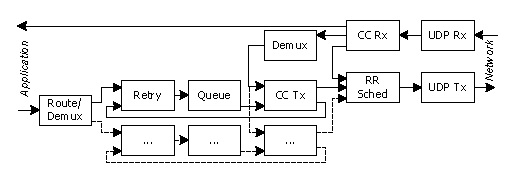
\includegraphics[width=\figurewidth]{ManyRetries}}
\centerline{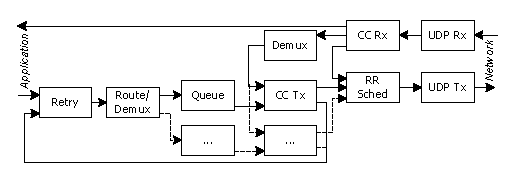
\includegraphics[width=\figurewidth]{SingleRetry}}
\caption{Persistent retries (top) vs.\ rerouting.}
\label{fig:RetryOrdering}
\end{figure}

P2~\cite{p2:sosp} is an overlay construction and
maintenance facility that uses a high-level declarative query language
to specify properties of overlay networks.   P2 dynamically translates
overlay specifications into Click-like~\cite{click-tocs} dataflow
networks, which are executed to maintain the overlay network.  A P2
dataflow network on a particular node consists of C++ objects
representing dataflow elements, with bindings between such objects
corresponding to arcs on the dataflow graph.  

Like Click, dataflow arcs between
elements pass data items via ``push'' or ``pull'' function calls.
However, P2 is primarily a query processor rather than an IP router. 
Unlike Click, P2 passes relational tuples rather than IP packets.
Furthermore, since P2 elements often produce and consume tuples via
computation rather than passing them through, P2 dataflows stop and
start more frequently and thus have more complex inter-element
synchronization and scheduling mechanims. 

P2 has a wide repertoire of dataflow element classes, including
operators necessary for performing relational query plan operations
(joins, aggregations, etc.) over tuples in both streams (e.g., from
the network) and local soft-state tables. 

P2 extends the dataflow model into the network stack, which is responsible
for inter-node tuple transfer.  Dataflow elements handle congestion
control, marshaling, packet scheduling, and demultiplexing.  Our
initial motivations for this novel design were ease of implementation
and consistency with the rest of the system, but we have come to
recognize its value as an abstraction for configuring transport protocols.  In the
following sections we show examples of the use of P2 dataflow elements
to address the issues identified in Section~\ref{sec:whatsdifferent}
by selective reordering and substitution.

\subsection{Sending Retries Down Alternate Paths}

Our first example allows an application to retry transmission of a
message to a potentially different destination.
Fig.~\ref{fig:RetryOrdering} shows two dataflow graphs, each of which
represents a possible configuration of transport protocol elements in
P2.  Broadly, packets to be sent move from left to right, and received
packets move from right to left.  For simplicity we do not show
whether bindings between elements are ``push'' or ``pull,'' and in
some cases we have collapsed chains of elements into a single box
where keeping them separate would not have aided comprehension.    

The upper diagram in Fig.~\ref{fig:RetryOrdering} shows conventional
TCP-like behavior for a P2P system.  A packet to be sent first passes
through a ``route/demux'' element which uses the overlay's routing
table to pick a next-hop destination, and hands the packet to a
per-neighbor retry element which enqueues it.  A packet is removed
from the head of this queue by a per-neighbor transmit-side congestion
control element (``CC Tx''), which in turn is scheduled by a global
round-robin element that pulls packets from the ``CC Tx'' elements
and sends them to the socket. 

Conversely, incoming packets from the network are pushed to a
receive-side congestion control element (``CC Rx'').
Incoming application data is acknowledged via the element's
path back to the round-robin scheduler, and pushed to the application.
Incoming acknowledgements from peers are demultiplexed and sent to the
appropriate ``CC Tx'' elements (to maintain congestion state), which
subsequently signal the retry elements (to remove data from the retry queue). 

\begin{figure*}[ht]
\centerline{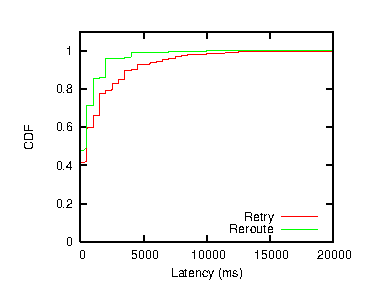
\includegraphics[scale=\graphscale]{results/latencyCDF.eps}
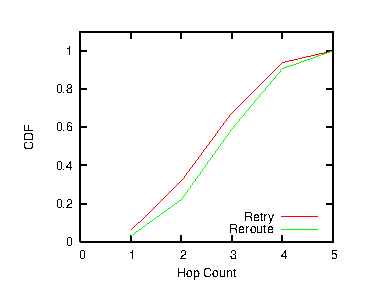
\includegraphics[scale=\graphscale]{results/hopCDF.eps}
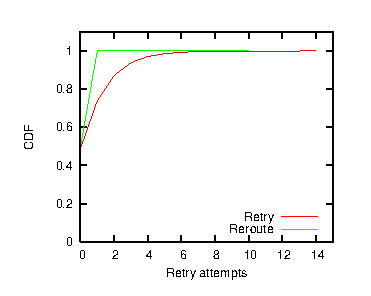
\includegraphics[scale=\graphscale]{results/retryCDF.eps}}
\caption{Comparing retry policies for Chord: (a) latency, (b) hop
  count, (c) retries.}
\label{fig:retry}
\end{figure*}

The lower diagram in Fig.~\ref{fig:RetryOrdering} shows how to
achieve behavior more like Bamboo, where successive retries may be
sent to different destinations. We simply move the retry element to
the head of the dataflow ahead of the route/demux element, which causes
each retransmission to perform a new route lookup.  Not shown is the
logic by which the route lookup has access to congestion and loss
statistics about neighbors -- this information is maintained as a P2
table, and the policy by which the route/demux element uses this
information to select a destination is likely to be
application-specific.  Note, however, that apart from expressing such 
preferences, no new code has to be written to achieve the desired behavior. 

%% Applications gain routing freedom (\S~\ref{sec:routingFreedom}) when we
%% allow them to route each retransmission of a dropped tuple over a
%% different path.  We illustrate how we can implement the traditional
%% TCP-like retry policy in our system, and how we can modify that
%% implementation for alternate-path retries in
%% Figure~\ref{fig:RetryOrdering}.  We first describe the common parts of the
%% two dataflow diagrams and then explain their differences.

%% In these simplified dataflow diagrams, the Application (at the left of
%% the graph) acts both as a producer and a consumer of tuple traffic.  A
%% tuple produced by the Application is pushed towards the right through
%% the transmission-side transport logic (to be described shortly). It is
%% then sent out via a round-robin tuple scheduler, marked ``RR Sched,'' to
%% the ``UDP Tx'' element for marshaling and transmission.  Incoming
%% traffic from the network is received by the ``UDP Rx'' element,
%% unmarshaled, and then pushed to the receive-side congestion control
%% element (``CC Rx'').  If the received tuple is an acknowledgment, it is
%% demultiplexed to the appropriate transmission-side congestion control
%% element, where it acknowledges some outstanding tuple~\footnote{This is
%% further signaled back to a ``Retry'' element to release memory resources
%% held for retransmission.}.  If it is instead a data tuple, it is sent
%% directly to the Application all the way to the left, and an
%% acknowledgment is sent out via the outoing tuple scheduler (via the
%% aforementioned ``RR Sched'' element).

%% The top dataflow diagram illustrates the traditional case where the next
%% hop of a tuple is decided (in the ``Route/Demux'' element) and
%% \emph{then} sent for reliable transmission. According to its
%% destination, the tuple is demultiplexed to the appropriate strand of
%% ``Retry,'' ``Queue,'' and ``CC Tx'' elements (one strand per
%% destination). The ``Retry'' element remembers state about the outgoing
%% tuple for potential retransmissions and pushes it to the following
%% ``Queue'' to await a downstream pull from the Network.  When the
%% transmission-side congestion control element ``CC Tx'' is ready to send,
%% it forwards the tuple toward transmission via the tuple scheduler.  ``CC
%% Tx'' represents any particular congestion control such as sender-based
%% (window) or receiver-based (TFRC) algorithms (\S~\ref{sec:substitution}). It detects tuple loss,
%% which it signals back to the ``Retry'' element. The Retry element, upon
%% receiving a loss signal, pushes the tuple again to the ``Queue.''

%% In the bottom dataflow diagram, although the functionality of individual
%% elements is the same, their arrangement in the flow is such that a
%% single ``Retry'' element precedes the ``Route/Demux'' element. As above,
%% the ``Retry'' element remembers tuples passing through it.  However, a
%% tuple acquires its next-hop destination afterwards, as it passes through
%% the ``Route/Demux'' element, and is then routed to the
%% destination-specific transmission strand of ``Queue'' and ``CC Tx''
%% elements.  The ``CC Tx'' element signals loss all the way to the common
%% ``Retry'' element, which retransmits a stored tuple downstream to the
%% ``Route/Demux'' element again.  Route selection at the routing element
%% can be as simple as choosing some other path or as complex as taking
%% into account the state of the congestion control
%% elements~\footnote{\note{P: I don't think we need to say this. Who knows
%% how we'll implement this in practice, including dumping CC state onto a
%% table and making the route element select from that table...}A control
%% path from congestion control to Retry would need to be setup in the
%% dataflow in order to take into account the congestion control element
%% state in retry path selection.}.

Figure~\ref{fig:retry} shows the results of a highly artificial
experiment comparing the performance of the two dataflow graphs.  We
build a very small (32-node) Chord network.  One 
particular node in the network performs 1 lookup per second to a
random key.  A lossy link (50\% drop rate) is placed between that lookup node and its
furthest finger table entry.
%% ~\footnote{The finger table is a routing table used 
%% by a node to greedily route lookups along the Chord ring topology. The
%% largest finger table entry covers half the key space distance along
%% the Chord ring.}
This experiment is, of course, simplistic in the extreme, but it
at least serves to isolate the effect of this change to the transport
protocol.

The results are unsurprising, and in line with much more rigorous
studies~\cite{rhea_usenix_2004,dabek_nsdi04}: moving retries ahead of
routing causes more hops to be traversed (since the path may not be
the best one available in the routing table), but the latency is
reduced (since we fail over links quickly).  Figure~\ref{fig:retry}
(c) clearly shows that this is achieved by reducing the number of
retries, since the lossy link is quickly avoided. 

%% We have implemented both versions of the dataflow graphs shown in
%% Figure~\ref{fig:RetryOrdering} and used them in an implementation of a
%% Chord network~\cite{chord}. A Chord network is an overlay network of
%% logarithmic diameter. The traffic that generally traverses a Chord
%% network is in the form of key lookups. The lookup key guides the routing
%% logic to make forward progress, through the intermediate hops, to the
%% ultimate overlay destination.

%% Figure~\ref{fig:retry} presents some initial results of the behavior of
%% both transport layer dataflow graphs. Our experimental setup uses $32$
%% nodes to form the overlay.  A particular node in the network
%% performs lookups at a rate of 1 lookup/sec. A lossy link is placed
%% between that lookup node and its first hop, which drops $50\%$ of all
%% traffic that traverses it.

%% Figure~\ref{fig:retry}(a) shows the cumulative distribution function
%% (CDF) for the end-to-end latency observed at the lookup node. The plot
%% shows that taking an alternate route following an initial failure
%% exhibits lower end-to-end latency. Figure~\ref{fig:retry}(b) and (c)
%% plot CDFs for the number of hops and retry attempts a lookup undergoes 
%% between its origin and final destination. Because with alternate routing some 
%% lookups might not take shortest available path, the hop count increases when 
%% retries are rerouted. The result presents a 
%% trade-off between latency and hop count. Overlay performance may benefit from 
%% a lower end-to-end latency, while security issues might make overlays that 
%% exhibit lower hop counts more desirable.\note{P: The previous two
%%   sentences are probably not useful here.}
%% The CDF for number of retries shows that 
%% rerouting around bad links results in fewer end-to-end retries in our
%% very simplistic example. An interesting repercussion of blind rerouting
%% via a lossy link is that it exacerbates queuing delays, since losses
%% cause the send window to shrink, inflating latency not only due to blind
%% persistence but also due to long waits in queues.

\subsection{Shared Congestion Control State}

An overlay STP-like behavior~\cite{dabek_nsdi04}, where a single
congestion window is maintained for all destinations can also be
generated without writing any additional code.  Figure~\ref{fig:STP}
illustrates how the same elements used above can be rearranged to
provide the functionality of STP using a single queue and congestion
control strand for all outgoing packets regardless of destination.

\begin{figure}
\centerline{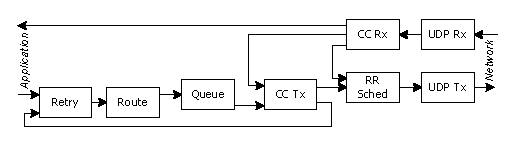
\includegraphics{STP}}
\caption{Shared congestion-control state for all destinations.}
\label{fig:STP}
\end{figure}

Note that the dataflow model makes it easy to combine orthogonal
functionality: we could have elected to perform retries ahead of
routing as above without requiring any new code. 

\subsection{Aggregation and late data choice}

Figure~\ref{fig:BufferedAggregation} shows an example of late data
choice for a distributed aggregation scenario, such as computing
the maximum or mean of a distributed set of values.  We move all
buffering in the data flow graph ``upstream,'' next to the
application. 

\begin{figure}
\centerline{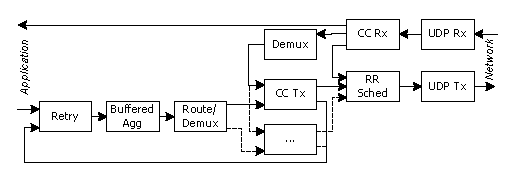
\includegraphics{BufferedAggregationRetries}}
\caption{Late data choice.}
\label{fig:BufferedAggregation}
\end{figure}

This simple change in the dataflow means that the number of aggregate
values sent by a node over time is equal to the load the network
is willing to handle.  When bandwidth is available, values are sent
out of the buffer as soon as they are produced, minizing the latency
with which the partial aggregates arrive at the next level of the
aggregation tree.  In the event of congestion, values remain in the
application buffers and are aggregating with any new values that
arrive, reducing bandwidth usage. 

\subsection{Heterogeneous transports}

Our final example briefly illustrates the ease with which different
combinations of transport protocol behaviors can be combined in an
application in a straightforward manner.  Figure
~\ref{fig:Classification} shows how different policies can be combined
at runtime, and choices made on a per-packet basis. 

\begin{figure}
\centerline{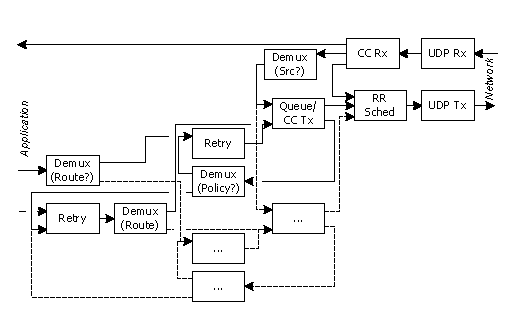
\includegraphics{Classification}}
\caption{Different, concurrent transport policies.}
\label{fig:Classification}
\end{figure}

% % % % % % % % % % % % % % % % % % % % % % % % % % % % % % % % % % 
\section{Related work}
\label{sec:related}

An early contribution in the decomposition of network protocols came
from the x-Kernel operating system~\cite{x-kernel}, in which network
services are handled by composable, user-level protocol objects. To
specify such objects, the project team developed the Morpheus~\cite{Morpheus}
programming language, which codifies valid protocol object compositions
and enables overhead-reducing optimizations.  Unlike our lightweight
elements, protocol objects in x-Kernel are complete protocol
implementations (i.e., TCP, Psync, BLAST), restricting their flexibility
to stacks that layer objects on top of one another.
With the slightly different motivation of making network protocol specifications more
\emph{readable}, Kohler et al.\ developed the Prolac Protocol
Language~\cite{prolac}. Prolac is an expression language, intended as for developing
complete protocols (e.g., TCP).

Sharing our high-level goals but taking a completely different approach,
Braden et al.~\cite{rba} propose a heap based protocol abstraction in
their Role-Based Architecture (RBA). 
In RBA, messages are addressed to role actors, instead of end-hosts. This allows 
middle boxes (e.g., firewalls, NAT boxes, caches, etc.), running as roles, to be addressed 
in message headers. Conceivably, RBA is an alternative to our dataflow
architecture for transport protocols although it seems ultimately
intended for larger-granularity actors, compared to our finer-grained
plumbing of protocol components before or after a multiplexer.
% 
% 
% Since the dataflow abstraction 
% represents a non-layered protocol design, we are also immune to issues surrounding 
% middle-box addressability. The focus of RBA is addressability of protocols and not on 
% better integration between application and protocol layers. We feel that 
% componentized protocols are better equipped to deal with application subtleties, i.e., 
% alternative route selection, buffer placement strategies, etc. 

Instead of offering flexibility via componentization, a number of
approaches expose the internals of monolithic protocol specifications,
making it easier to pick and choose which flexibility to enable and
which to suppress. 
Mogul et al.~\cite{unveiling} describe a put/get interface to the transport layer that allows for the setting
and querying of network protocol state.
The Datagram Congestion Control Protocol (DCCP)~\cite{dccp} builds a
transport ``suite'' that can flexibly alter its behavior
while remaining TCP-friendly. In both cases, the resulting protocol
instantiations are geared towards point-to-point communication, and
keep all pieces of the transport functionality within the same
``shell,'' making it harder to effect the flexible reordering of
components across traditional layer boundaries that we
propose in our work.

The software dataflow abstraction has long been used to model data
movement in the database literature, in particular in
networked and stream query engines~\cite{telegraphcq,aurora}, which
have an intimate relation to data-intensive networking.  More recently
it has been embraced for network
routers~\cite{click-tocs,handley05xorp}.  Many of the 
optimizations found in these systems are a direct result of using a
dataflow model, and the flexibility thereof.  Network
transport protocols can also benefit from a dataflow model, and in
this paper we have presented a few such examples.  An interesting
synergy may also exist between the flexibility we have seen in this paper
and database query optimization techniques, particularly {\em
  adaptive} approaches to reoptimizing live
dataflows~\cite{telegraphcq,babu-cidr05}.


% % % % % % % % % % % % % % % % % % % % % % % % % % % % % % % % % % 
\section{Conclusion}
\label{sec:discussion}

Overlay networks offer a new network model that applications are beginning 
to demand. This new communication medium brings with it a number of design 
decisions that go beyond the scope of a small number of monolithic
transport protocol services. Component based transport protocols
provide a natural replacement of black box protocol implementations,
with small processing units that can be arranged to form the desired
semantics. Besides flexibility, designing a system around small components promotes
good code reuse.

We embrace a dataflow architecture for our component-based transport
protocols.  Dataflows have been shown to provide good
data independence properties in many other systems, and are certainly
capable of supporting high-performance
operation~\cite{BrewerInktomi}. The flexibility of a
dataflow abstraction makes the rich set of optimizations afforded by
overlay networks easier to attain. Moreover, it provides an ideal glue
layer between the application and network, one which we have shown to
support fresh results and good synchronization properties. 

In the future, it may become important to ensure that component-based
transport 
protocols mimic the wire formats of existing transports, particularly
TCP.  This would ease interoperation with existing middleboxes, allowing
for example firewalls and NATs to maintain per-flow state obliviously.
Mimicking the particular timing characteristics of specific TCP
implementations, however, may prove more challenging.

Finally, a particularly challenging and ambitious next step for our exploration of this space
is the specification in a high-level language of \emph{desired properties}
for a particular instantiation of protocol components.  In P2, we define
and compile entire
application-level overlay dataflows from such declarative language specifications.
Consequently, this approach would allow us to redraw the
boundary between the overlay and the transport.



{\footnotesize
\bibliography{paper,rfcs}
}
\end{document}
